\documentclass[12pt, times new roman, a4paper]{article}
\linespread{1,5}
\usepackage[utf8]{inputenc}
\usepackage{graphicx}
\usepackage{listings}
\renewcommand{\figurename}{Gambar}

\begin{document}

\section{Teroi}

\subsection{Jenis variabel dan cara pemakaiannya}

\subsubsection{Variabel dengan tipe data angka}
nama = "adit"\\
kelas = "2c"\\
print "Nama : "nama\\
print "kelas : "kelas\\
\subsubsection{Variabel dengan tipe data teks}
umur = 19\\
npm = 1184090\\
print "Umur : "umur\\
print "NPM : "npm\\
\subsubsection{Variabel dengan tipe data boolean}
rajin = False\\
if(rajin):\\
	print "Anak anda : rajin"\\
else:\\
	print "Anak anda : kurang rajin"\\
	
\subsection{Input dari user dan output ke layar}
name = input('Masukkan nama: ')\\
Masukkan nama: Aditya\\
print(name)\\
Aditya\\

\subsection{Operator dasar aritmatika dan mengubah string ke integer dan sebaliknya}
\subsubsection{Operator dasar aritmatka}
(+) adalah operator penambahan\\
(-) adalah operator pengurangan\\
(*) adalah operator perkalian\\
(/) adalah operator pembagian(pecahan)\\
(//) adalah operator pembagian(dibulatkan kebawah)\\
(persen) adalah operator modulus\\
(**) adalah operator pemangkatan\\
\subsubsection{Mengubah string ke integer dan sebaliknya}
1. Mengubah string ke integer\\
a = "20"\\
b = 19\\
c = (int(a) + int(b))\\
print (c)\\
\begin{figure}[h]
	\centering
		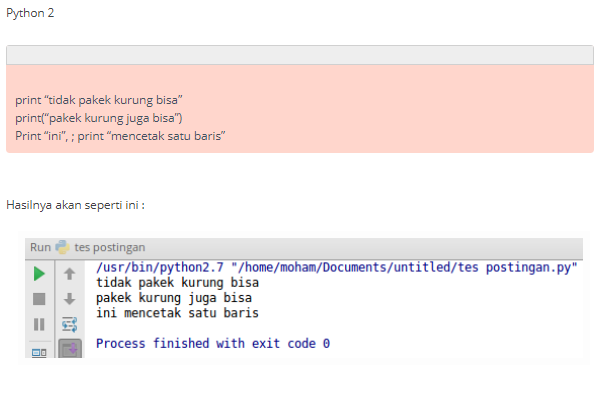
\includegraphics[scale=1.2]{Gambar/1}
	\caption{mengubah str ke int}
\end{figure}
\\
\\
2. Mengubah integer ke string\\
a = "aditya"\\
b = 19\\
c = (str(a) + str(b))\\
print (c)\\
\begin{figure}[h]
	\centering
		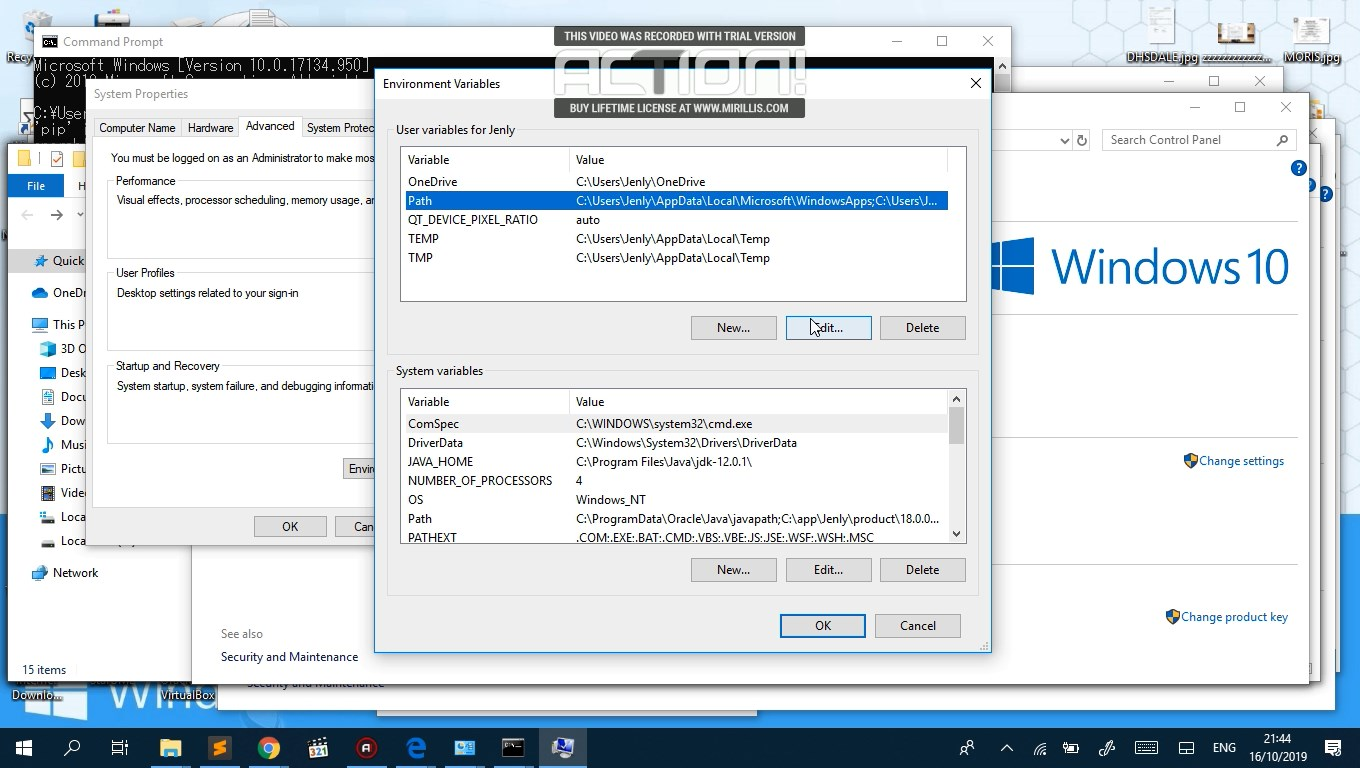
\includegraphics[scale=1]{Gambar/2}
	\caption{mengubah int ke str}
\end{figure}

\subsection{Perulangan (looping)}
\subsubsection{ While Loop}
While Loop adalah perulangan yang digunakan dalam bahasa pemprograman python dan akan dieksekusi selama kondisinya bernilai benar(true).\\
Count = 0\\
While (count < 9):\\
Print ’ The count is:’, count\\
Count = count +1\\
Print ("Good bye !")\\
\subsubsection{For Loop}
For Loop adalah perulangan pada python untuk mengulangi item dari
urutan apapun, seperti list atau string.\\
Contoh implementasi :\\
Angka =[1,2,3,4,5]\\
For x in angka:\\
Print(x)\\

\subsection{Kondisi}
Kondisi pada Python ada 3 yaitu :\\
\subsubsection{If}
IF yaitu kondisi yang bernilai benar atau salah. Jika nilai statementnya
bernilai benar maka statement akan dijalankan dan jika nilai statementnya
bernilai salah maka statement tidak akan dijalankan.\\
Contohnya yaitu :
\begin{verbatim}
X=1
IF x >0:
	Print("Nilai  %x adalah besar dari 0"% x)
#NIlai 1 adalah besar dari 0
\end{verbatim}
Kondisi diatas adalah bernilai true / benar, dimana nilai x(1) lebih besar
dari 0. Coba ubah kondisinya seperti berikut:
\begin{verbatim}
 X=1
IFx>2:
Print("Nilai %X adalah besar  dari 0" %x)
\end{verbatim}
Jika kita jalankan kode diatas maka python tidak akan menampilkan output apapun, karena sudah jelas bahwa kondisi diatas adalah bernilai false
/ salah.\\
\subsubsection{If-Else}
IF- Else yaitu jika kondisi bernilai true maka statemen didalam if akan
dieksekusi dan jika bernilai false maka statemen yang dieksekusi adalah
statemen didalam else.\\
Contohnya:
\begin{verbatim}
X=1
IF x> 5:
Print("Nilai %d adalah besar dari 5" % X)
Else:
Print("Nilai %d adalah kecil dari %" % X)
#Nilai 1 adalah kecil dari 5
\end{verbatim}
Sebaliknya, mari kita ubah nilai x menjadi 10 :\\
\begin{verbatim}
X=10
IF X >5:
Print("Nilai %d adalah besar dari 5" % X)
Else:
Print("Nilai %d adalah kecil dari 5" % X)
\end{verbatim}
\subsubsection{IF ELIF ELSE}
IF ELIF ELSE yaitu Kondisi Elif Kondisi Elif ini lanjutan dari percabangan kondisi if dengan kondisi elif ini kita bisa membuat kode program yang
akan menyeleksi beberapa kemungkinan yang bisa terjadi.\\
Contohnya:
\begin{verbatim}
x = 5
if x < 5:
	print("Nilai %d adalah kecil dari 5" % x )
elif x == 5 :
	print("Nilai %d adalah sama dengan 5" % x)
else :
	print("Nilai %d adalah besar dari 5" % x)
\end{verbatim}
 
\subsection{Jenis error yang sering ditemui pada python}
\subsubsection{ TypeError: unsupported operand type(s) for +: ’int’ and ’str’}
cara mengatasinya yaitu: menggunakan casting operand kedua menjadi
integer\\
\subsubsection{TypeError: can only concatenate str (not ”int”) to str}
cara mengatasinya yaitu: menggunakan casting operand kedua menjadi
string\\

\subsection{Try Except}
Try except adalah bentuk penanganan error yang terdapat dalam python. Contoh penggunaannya : Setiap bilangan yang dibagi 0 akan terjadi error karena
sudah ketentuan dari awal dan tidak bisa di eksekusi tetapi dengan menggunakan try except dapat di eksekusi walaupun akan terjadi error seperti contoh
dibawah ini :\\
\begin{verbatim}
X=0
Try:
X=9/0
Except exception,e;
Print e

Print x=1
\end{verbatim}
Maka akan muncul peringatan error integer division or modulo by zero 1\\

\section{Ketrampilan Pemrograman}


\subsection{soal 2}
\lstinputlisting[language=Python]{src/2.py}
\subsection{soal 3}
\lstinputlisting[language=Python]{src/3.py}
\subsection{soal 4}
\lstinputlisting[language=Python]{src/4.py}
\subsection{soal 5}
\lstinputlisting[language=Python]{src/5.py}
\subsection{soal 6}
\lstinputlisting[language=Python]{src/6.py}
\subsection{soal 7}
\lstinputlisting[language=Python]{src/7.py}
\subsection{soal 8}
\lstinputlisting[language=Python]{src/8.py}
\subsection{soal 9}
\lstinputlisting[language=Python]{src/9.py}
\subsection{soal 10}
\lstinputlisting[language=Python]{src/10.py}
\subsection{soal 11}
\lstinputlisting[language=Python]{src/11.py}


\end{document}